% 可选：插入section_5_2.tex的预处理段之后、末段之前。
% 若正文篇幅有限，可将此图移至附录。
图~\ref{fig:p1_raw_timeline}展示了一条样本经预处理后的声画时间记录。上方为从抽样序列中选取的实际视频帧，下方为同一片段的单声道音频波形，两者均以视频起点为时间原点。给定转写在此阶段仅保留文本内容，尚无词级起止时间，因而仍需在后续处理中估计词边界，建立文本与声画的对应关系。

\begin{figure}[htbp]
    \centering
    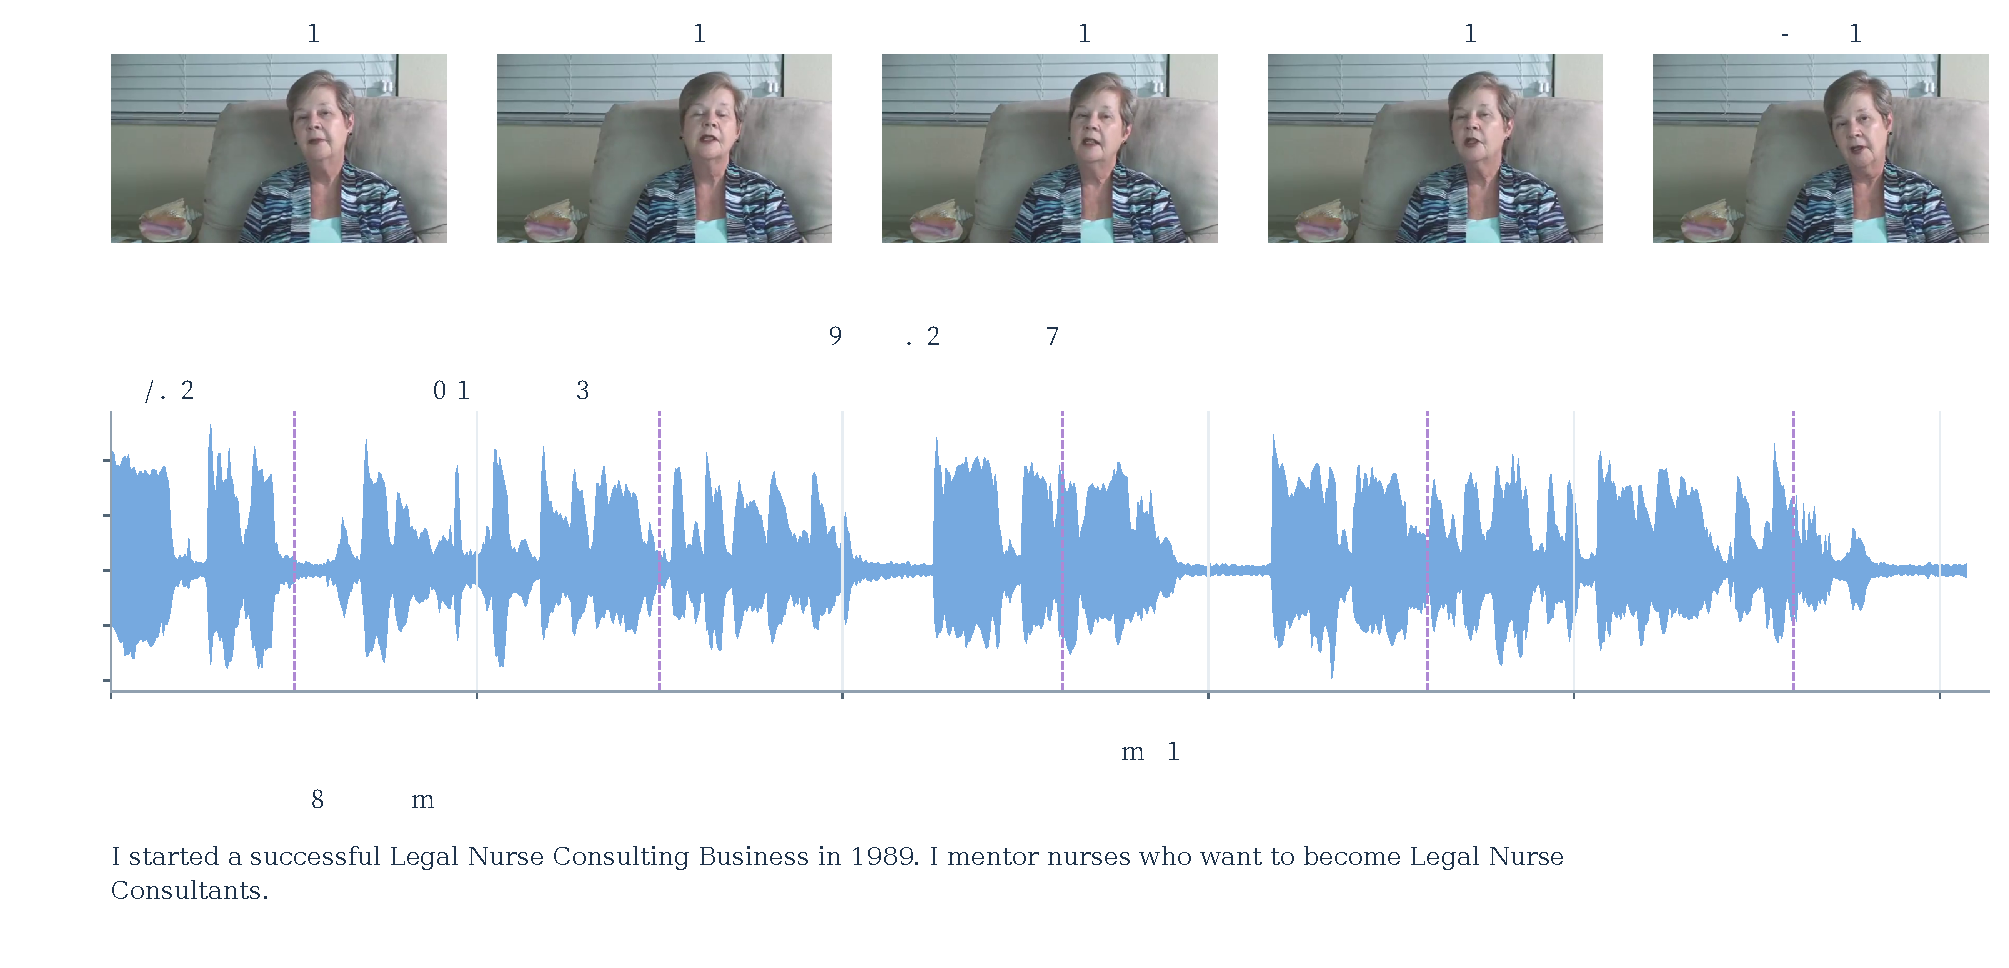
\includegraphics[width=\textwidth]{figures/fig_5_2_raw_timeline.pdf}
    \caption{单条样本预处理后的声画时间记录。示例编号为 \texttt{-egA8-b7-3M\$\_\$1}。为便于显示，波形以每10毫秒内的最小值与最大值构成包络；虚线表示上方视频帧的实际时刻，不表示词边界。}
    \label{fig:p1_raw_timeline}
\end{figure}
